\documentclass[12pt,a4paper]{article}
\usepackage[utf8]{inputenc}
\usepackage[T1]{fontenc}
\usepackage{amsmath}
\usepackage{amssymb}
\usepackage{geometry}
\usepackage{setspace}
\usepackage{parskip}
\usepackage{enumitem}
\usepackage{booktabs}
\usepackage{longtable}
\usepackage{array}
\usepackage{xcolor}
\usepackage{hyperref}
\usepackage{float}
\usepackage{tikz}
\usetikzlibrary{arrows.meta,positioning,calc}
\usepackage{fancyhdr}
\usepackage{titlesec}
\usepackage{tcolorbox}
\tcbuselibrary{skins,breakable}

\geometry{left=2.5cm,right=2.5cm,top=2.5cm,bottom=2.5cm,headheight=14.5pt}
\onehalfspacing
\hypersetup{colorlinks=true,linkcolor=black,urlcolor=blue,pdftitle={Guía de Estudio para la Sustentación - Sistema Integral de Gestión de Eventos},pdfauthor={Samuel Contreras}}

\definecolor{azul}{RGB}{31,78,121}
\definecolor{gris}{RGB}{242,242,242}
\definecolor{grisoscuro}{RGB}{80,80,80}
\definecolor{verde}{RGB}{39,120,70}
\definecolor{naranja}{RGB}{230,126,34}
\definecolor{morado}{RGB}{106,27,154}
\definecolor{rojo}{RGB}{176,42,42}

\titleformat{\section}{\Large\bfseries\color{azul}}{\thesection.}{0.5em}{}
\titleformat{\subsection}{\large\bfseries}{\thesubsection.}{0.5em}{}
\renewcommand{\contentsname}{Índice}
\renewcommand{\figurename}{Figura}
\renewcommand{\tablename}{Tabla}

\pagestyle{fancy}
\fancyhf{}
\fancyhead[L]{Sistema Integral de Gestión de Eventos}
\fancyhead[R]{Guía de Estudio --- Sustentación}
\fancyfoot[C]{\thepage}

\newtcolorbox{pregunta}[1][]{
  colback=blue!4,colframe=azul,boxrule=0.5pt,arc=2pt,
  left=6pt,right=6pt,top=4pt,bottom=4pt,breakable,#1
}
\newtcolorbox{alerta}[1][]{
  colback=orange!6,colframe=naranja,boxrule=0.5pt,arc=2pt,
  left=6pt,right=6pt,top=4pt,bottom=4pt,breakable,#1
}

\begin{document}

\begin{titlepage}
\centering
\vspace*{2cm}
{\Huge\bfseries Sistema Integral de Gestión de Eventos\par}
\vspace{0.7cm}
{\Large Arquitectura de Software\par}
\vspace{1.2cm}
{\Large\bfseries Guía de Estudio para la Sustentación\par}
\vspace{2cm}
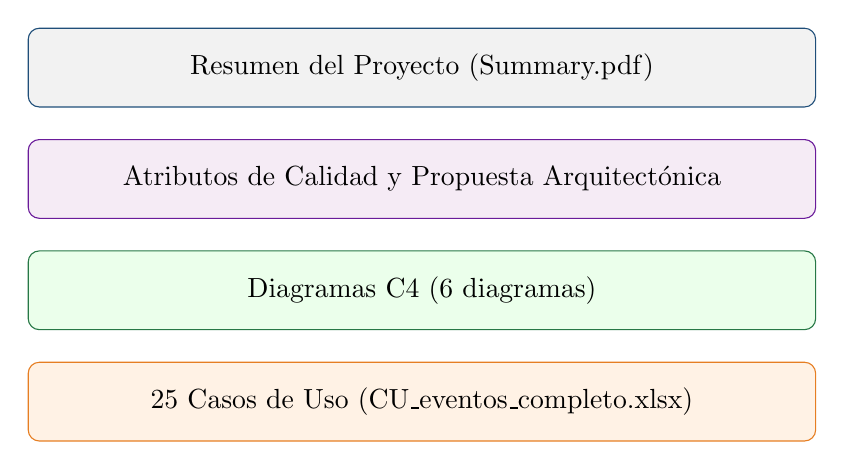
\begin{tikzpicture}
\node[draw=azul,rounded corners,fill=gris,minimum width=10cm,minimum height=1cm,align=center]
{Resumen del Proyecto (Summary.pdf)};
\node[draw=morado,rounded corners,fill=violet!8,minimum width=10cm,minimum height=1cm,below=0.4cm of current bounding box.south,align=center]
{Atributos de Calidad y Propuesta Arquitectónica};
\node[draw=verde,rounded corners,fill=green!8,minimum width=10cm,minimum height=1cm,below=0.4cm of current bounding box.south,align=center]
{Diagramas C4 (6 diagramas)};
\node[draw=naranja,rounded corners,fill=orange!10,minimum width=10cm,minimum height=1cm,below=0.4cm of current bounding box.south,align=center]
{25 Casos de Uso (CU\_eventos\_completo.xlsx)};
\end{tikzpicture}
\vfill
\textit{Documento de preparación personal --- no es un entregable del curso.}\\[4pt]
\textit{Explica, archivo por archivo, qué hay en \texttt{Submission/} y qué debes poder responder.}
\vfill
\begin{tabular}{rl}
\textbf{Materia:} & Arquitectura de Software\\
\textbf{Estudiante:} & Samuel Contreras\\
\textbf{Fecha:} & Agosto de 2026
\end{tabular}
\end{titlepage}

\tableofcontents
\newpage

\section{Cómo usar esta guía}

Este documento \textbf{no se entrega al profesor} --- vive en \texttt{Defense/} para que estudies
antes de sustentar, no en \texttt{Submission/}. Repasa lo que dice el reglamento del curso sobre la
sustentación (Clase 1, \texttt{Work/Notes/01...md}):

\begin{itemize}
\item Dura \textasciitilde 1 hora, \textbf{sin orden fijo}: descripción general de lo entregado,
requisitos/diseño/implementación/pruebas, demo del prototipo. \textbf{Cada integrante demuestra su
parte.}
\item Como se usó IA generativa para redactar código y documentos, \textbf{cada estudiante es
responsable de lo que la IA generó}: debes poder explicar cada término usado, la razón detrás de
cada decisión de diseño, y --- cuando haya código --- qué hace cada línea. El profesor puede
verificarlo a su discreción y la nota se ve afectada si no puedes responder.
\end{itemize}

Por eso cada sección de esta guía no solo resume el contenido del archivo, sino que incluye
\textbf{preguntas que el profesor podría hacer} (recuadros azules) y \textbf{puntos delicados que
debes tener listos} (recuadros naranjas: inconsistencias conocidas, decisiones que fueron
sugeridas por el asistente de IA y que el equipo debería revisar, temas sin resolver).

\section{Mapa general: cómo se relacionan los 4 archivos}

\texttt{Submission/} tiene cuatro archivos. No son independientes entre sí: cada uno mira el mismo
sistema desde un ángulo distinto, del más general al más detallado.

\begin{longtable}{p{3cm}p{3.3cm}p{7.5cm}}
\toprule
\textbf{Archivo} & \textbf{Rol} & \textbf{Qué responde}\\
\midrule
\endfirsthead
\toprule
\textbf{Archivo} & \textbf{Rol} & \textbf{Qué responde}\\
\midrule
\endhead
Summary.pdf & Resumen ejecutivo & ``¿Qué hace el sistema y qué parte hiciste tú?'' --- las 4
interfaces, los actores, y los 5 CU de personal (CU-006 a CU-010) con su interfaz principal.\\[0.4em]
ArchitecturalProposal.pdf & Atributos de calidad + arquitectura & ``¿Por qué eligieron esta
arquitectura?'' --- prioriza atributos de calidad, propone microservicios + infraestructura, y
explica cómo cada decisión satisface cada atributo. Incluye el caso complejo de Evacuación
(CU-010).\\[0.4em]
C4Diagrams.pdf & Los mismos componentes, dibujados & ``¿Cómo se ve esa arquitectura?'' --- 6
diagramas C4 hechos en draw.io (Contexto, Contenedores, Componentes, Panorama de Sistemas,
Secuencia, Despliegue), cada caja con nombre + tipo/tecnología + descripción, todos validados
contra el checklist oficial.\\[0.4em]
CU\_eventos\_completo.xlsx & Las 25 fichas de casos de uso & ``¿Qué hace exactamente el sistema,
paso a paso?'' --- una ficha por caso de uso con flujo básico, alternos, excepciones, atributos de
calidad e infraestructura.\\
\bottomrule
\caption{Los 4 archivos de Submission y cómo se relacionan.}
\end{longtable}

\begin{alerta}
\textbf{Ojo:} los tres documentos en prosa (\textit{Summary}, \textit{ArchitecturalProposal},
\textit{C4Diagrams}) tienen como autor a Samuel Contreras --- son el aporte individual que
corresponde defender con más detalle. El Excel de 25 CU es del equipo completo: tus 5 propios
(CU-006 a CU-010) los debes dominar a fondo; del resto basta con entender el panorama general
(quién los hizo, qué módulo cubren) porque en la sustentación cada integrante presenta lo suyo.
\end{alerta}

\section{Summary.pdf --- Resumen del Proyecto}

\subsection{Qué es y de dónde sale}

Compilado desde \texttt{Work/Summary.tex}. Es la primera pieza que alguien debería leer: plantea el
problema (procesos de un evento hoy dispersos, sin trazabilidad), y cómo el sistema lo resuelve con
\textbf{una app web (dos portales)} y \textbf{una app móvil (dos variantes)}, todas contra el mismo
backend.

\subsection{Estructura del documento}

\begin{enumerate}
\item \textbf{Idea general y problema que resuelve.}
\item \textbf{Arquitectura de interfaces} --- tabla de las 4 interfaces (Portal Web Administrativo,
Portal Web Cliente, App Móvil Cliente, App Móvil Personal), su audiencia y qué hace cada una.
\item \textbf{Actores del sistema} --- Cliente, Organizador, Empleado, Administrador, Supervisor de
emergencia, más los 2 sistemas externos (pasarela de pagos, notificaciones).
\item \textbf{Casos de uso asignados y su interfaz} --- tus 5 CU (CU-006 a CU-010), con cuál
interfaz usa cada uno.
\item \textbf{Atributos de calidad priorizados} --- versión resumida de la tabla completa de
\textit{ArchitecturalProposal.pdf}.
\item \textbf{Arquitectura de backend} --- API Gateway, microservicios, Redis, colas, pasarela de
pagos, con un diagrama de bloques.
\item \textbf{Documentación entregada (modelo C4)} --- referencia cruzada a \textit{C4Diagrams.pdf}.
\end{enumerate}

\subsection{Tus 5 casos de uso (lo que más te van a preguntar)}

\begin{longtable}{p{2.1cm}p{5.6cm}p{5.8cm}}
\toprule
\textbf{CU} & \textbf{Qué hace} & \textbf{Interfaz principal}\\
\midrule
\endfirsthead
\toprule
\textbf{CU} & \textbf{Qué hace} & \textbf{Interfaz principal}\\
\midrule
\endhead
CU-006 \newline \textit{(complejo)} & Mercado secundario: publicar, comprar, pagar, transferir
propiedad, invalidar/regenerar QR. & Portal Web Cliente (+ App Móvil Cliente recibe el QR nuevo).\\[0.4em]
CU-007 & CRUD de empleados + asignación a eventos (rol, horario, conflictos). & Portal Web
Administrativo (confirmación desde App Personal).\\[0.4em]
CU-008 & Solicitud, búsqueda de reemplazo y aprobación de cambios de turno. & App Personal
(solicitud) + Portal Administrativo (aprobación).\\[0.4em]
CU-009 & Control de asistencia por QR/credencial y cálculo de horas. & App Móvil del Personal.\\[0.4em]
CU-010 \newline \textit{(complejo)} & Activar, coordinar y cerrar un protocolo de evacuación en
tiempo real. & Portal Administrativo (activa) + ambas apps móviles (reciben alertas).\\
\bottomrule
\caption{Tus 5 casos de uso, resumidos.}
\end{longtable}

\begin{pregunta}
\textbf{Posibles preguntas del profesor:}
\begin{itemize}
\item ``¿Por qué CU-010 es el caso complejo y no otro de los suyos?'' --- Porque es el único que
toca las \textbf{tres interfaces a la vez} (web administrativo para activar/monitorear, ambas apps
para recibir alertas), tiene múltiples flujos alternos y de excepción (ruta bloqueada, zona
congestionada, cambio de nivel de emergencia), y exige atributos de calidad no triviales
(disponibilidad, tiempo real, seguridad) resueltos con infraestructura real (colas de alta
prioridad, notificaciones multicanal).
\item ``¿Por qué separaron CU-007 (gestión de personal) de CU-008 (cambios de turno) en vez de un
solo CU?'' --- Son procesos distintos con actores y momentos distintos: CU-007 ocurre en la
planeación (antes del evento), CU-008 ocurre durante la operación cuando surge un imprevisto.
\item ``¿Qué pasa si dos empleados intentan tomar el mismo turno de reemplazo al mismo tiempo?''
--- Es exactamente el tipo de conflicto de concurrencia que se resuelve verificando disponibilidad
antes de aprobar (CU-008, paso de verificación) --- puedes conectarlo con el mismo patrón de
bloqueo temporal que usa CU-006 con Redis.
\end{itemize}
\end{pregunta}

\section{ArchitecturalProposal.pdf --- Atributos de Calidad y Propuesta Arquitectónica}

\subsection{Qué es y de dónde sale}

Compilado desde \texttt{Work/ArchitecturalProposal.tex}. Es el documento \textbf{más importante
para la sustentación} porque conecta \textit{por qué} con \textit{qué}: parte de los atributos de
calidad priorizados y termina explicando, atributo por atributo, cómo la arquitectura propuesta lo
satisface. Es también donde vive el \textbf{Resumen de decisiones arquitectónicas} que ahora está
migrado (con alternativas y riesgos) a \texttt{Work/BitacoraArquitectonica.md}.

\subsection{Estructura del documento}

\begin{enumerate}
\item \textbf{Introducción} --- 4 interfaces, dominios que centraliza el sistema.
\item \textbf{Contexto y alcance} --- 7 dominios (boletería, mercado secundario, parqueaderos,
logística, administración, personal, emergencias).
\item \textbf{Interfaces del sistema} --- detalle de qué hace cada una de las 4.
\item \textbf{Atributos de calidad priorizados} --- tabla con \textbf{Prioridad / Atributo /
Justificación} para 10 atributos.
\item \textbf{Arquitectura propuesta} --- diagrama de bloques completo: 4 clientes $\to$ API
Gateway $\to$ Balanceador $\to$ 6 microservicios $\to$ Redis/Colas/BD $\to$ servicios externos.
\item \textbf{Infraestructura de soporte} --- Redis, RabbitMQ/Kafka, bases de datos por dominio.
\item \textbf{Servicios externos} --- pasarela de pagos, notificaciones.
\item \textbf{Cómo la arquitectura satisface los atributos de calidad} --- una subsección por
atributo (10 en total), explicando el mecanismo concreto.
\item \textbf{Caso complejo: Gestión de Evacuación ante Emergencias} --- objetivo, actores, flujo
principal (15 pasos), alternos, excepciones, atributos de calidad del caso.
\item \textbf{Comunicación durante una emergencia} --- diagrama de secuencia simplificado.
\item \textbf{Relación entre interfaces y microservicios} --- tabla resumen.
\item \textbf{Resumen de decisiones arquitectónicas} --- tabla Decisión / Problema / Atributos.
\item \textbf{Conclusión.}
\end{enumerate}

\subsection{Tabla de atributos de calidad (memorízala con su prioridad)}

\begin{longtable}{p{2.4cm}p{2.7cm}p{7.6cm}}
\toprule
\textbf{Prioridad} & \textbf{Atributo} & \textbf{Por qué}\\
\midrule
\endfirsthead
\toprule
\textbf{Prioridad} & \textbf{Atributo} & \textbf{Por qué}\\
\midrule
\endhead
Alta & Consistencia & Una entrada no puede tener dos dueños ni venderse dos veces a la vez.\\
Alta & Disponibilidad & Crítico en ventas, ingreso masivo, operación y emergencias.\\
Alta & Seguridad & Datos personales, pagos, QR, permisos por rol.\\
Alta & Rendimiento & Miles de operaciones concurrentes con respuesta rápida.\\
Media-Alta & Tiempo real & Aforo, entradas, personal, parqueaderos y emergencias casi al instante.\\
Media & Escalabilidad & Poder aumentar instancias de los servicios con más demanda.\\
Media & Trazabilidad & Auditar transferencias, pagos, accesos, turnos, emergencias.\\
Baja-Media & Usabilidad & Interfaces adaptadas a cada tipo de usuario.\\
Baja-Media & Mantenibilidad & Un dominio cambia sin afectar innecesariamente a los demás.\\
Baja-Media & Portabilidad & Misma lógica de negocio, consumida desde web y apps.\\
\bottomrule
\caption{Los 10 atributos de calidad priorizados.}
\end{longtable}

\subsection{Las 9 decisiones arquitectónicas (tabla resumen)}

\begin{longtable}{p{3.4cm}p{4.6cm}p{4.6cm}}
\toprule
\textbf{Decisión} & \textbf{Qué problema resuelve} & \textbf{Atributos que favorece}\\
\midrule
Microservicios & Separación de dominios y escalamiento independiente & Escalabilidad,
mantenibilidad, rendimiento\\
API Gateway & Punto central de acceso y seguridad & Seguridad, mantenibilidad\\
Balanceador de carga & Distribución de solicitudes entre instancias & Disponibilidad, rendimiento\\
Redis & Acceso rápido y bloqueo temporal de concurrencia & Consistencia, tiempo real, rendimiento\\
RabbitMQ/Kafka & Procesamiento asíncrono desacoplado & Rendimiento, escalabilidad\\
BD por servicio & Evitar acoplamiento de datos entre dominios & Mantenibilidad, escalabilidad\\
Notificaciones & Comunicación desacoplada del flujo principal & Rendimiento, tiempo real\\
Pasarela de pagos & Delegar transacciones externas a un tercero especializado & Seguridad,
consistencia\\
Interfaces especializadas & Adaptar cada superficie al tipo de usuario & Usabilidad, portabilidad\\
\bottomrule
\caption{Las 9 decisiones y qué resuelven.}
\end{longtable}

\begin{pregunta}
\textbf{Posibles preguntas del profesor (y cómo responderlas con una frase):}
\begin{itemize}
\item \textit{``¿Por qué microservicios y no un monolito?''} --- Porque el equipo necesita escalar
de forma independiente el servicio con más demanda (p. ej. Entradas en una apertura de venta) sin
sobre-aprovisionar los demás dominios, y porque cada equipo/subgrupo del proyecto es dueño de un
dominio distinto (boletería, personal, pedidos, logística, parqueaderos) --- separarlos en
servicios reduce el acoplamiento entre lo que hace cada subequipo.
\item \textit{``Expliqué el teorema CAP aplicado a su sistema.''} --- Ante una partición de red, el
sistema debe elegir entre Consistencia y Disponibilidad para cada operación: en el checkout de una
entrada se prioriza \textbf{Consistencia} (mejor rechazar una compra que vender la misma entrada
dos veces); en la consulta de eventos se prioriza \textbf{Disponibilidad} (mejor mostrar datos
ligeramente desactualizados que no mostrar nada).
\item \textit{``¿Por qué Redis y no un lock a nivel de base de datos?''} --- Redis resuelve el
bloqueo en memoria, con latencia mucho menor que un lock transaccional en la base de datos, algo
crítico cuando miles de usuarios compiten por la misma entrada en segundos.
\item \textit{``¿Qué pasa si Redis se cae?''} --- Es un riesgo real y vale admitirlo: sin el
bloqueo temporal, dos compradores podrían iniciar el checkout de la misma entrada; la mitigación es
que la validación final de propiedad ocurre también contra la base de datos transaccional antes de
confirmar el pago, y Redis se desplegaría en modo clúster/Sentinel (ver \textit{Diagrama de
Despliegue} en \textit{C4Diagrams.pdf}) para reducir la probabilidad de caída total.
\item \textit{``¿Por qué una cola de mensajes para las notificaciones y no una llamada directa?''}
--- Para que un fallo o demora del proveedor de notificaciones no bloquee ni haga fallar la
operación principal (compra, transferencia); la cola reintenta sin afectar al usuario.
\end{itemize}
\end{pregunta}

\begin{alerta}
\textbf{Punto delicado:} este documento no incluye todavía un \textbf{Árbol de Utilidad} (Utility
Tree) formal para justificar los ASR más prioritarios, técnica enseñada en la Clase 5. Está en
\texttt{TASKS.md} como pendiente explícito. Si el profesor pregunta por él, la respuesta honesta es
que la priorización de atributos de calidad sí está hecha (la tabla de arriba), pero aún no en el
formato explícito de árbol con escenarios (H,H).
\end{alerta}

\section{C4Diagrams.pdf --- Diagramas de Arquitectura (Modelo C4)}

\subsection{Qué es y de dónde sale}

Compilado desde \texttt{Work/C4Diagrams.tex}. Complementa a \textit{ArchitecturalProposal.pdf}: en
vez de explicar con palabras, \textbf{dibuja} la misma arquitectura en 6 diagramas siguiendo el
modelo C4 de Simon Brown, cada uno validado contra el checklist oficial de
\href{https://c4model.com/diagrams/checklist}{c4model.com/diagrams/checklist}. Los 6 diagramas se
elaboraron en \href{https://app.diagrams.net/}{draw.io} (no como código tikz) siguiendo dos
indicaciones del profesor: cada caja muestra nombre, tipo/tecnología y una breve descripción, y el
antiguo Diagrama Dinámico se reemplazó por un diagrama de secuencia UML. Los archivos fuente
\texttt{.drawio} están en \texttt{Work/Diagrams/}.

\subsection{Los 6 diagramas, uno por uno}

\begin{longtable}{p{2.6cm}p{2.1cm}p{7.9cm}}
\toprule
\textbf{Diagrama} & \textbf{Nivel} & \textbf{Qué muestra}\\
\midrule
\endfirsthead
\toprule
\textbf{Diagrama} & \textbf{Nivel} & \textbf{Qué muestra}\\
\midrule
\endhead
Contexto & 1 & El sistema como caja negra frente a 5 roles (Cliente, Organizador, Empleado,
Administrador, Supervisor de emergencia) y 2 sistemas externos (pasarela de pagos, notificaciones).\\[0.4em]
Contenedores & 2 & Zoom adentro: 2 apps (web + móvil), API Gateway, 5 microservicios, Redis, cola de
mensajes, bases de datos.\\[0.4em]
Componentes & 3 & Zoom al microservicio más complejo (Entradas y Mercado Secundario, CU-006):
Controlador API, Servicio de Publicación, Gestor de Concurrencia, Procesador de Pagos, Generador de
QR, Repositorio, Publicador de Eventos.\\[0.4em]
Panorama de Sistemas & Auxiliar & Zoom hacia \textbf{afuera}: el sistema junto a otros sistemas de
la organización (Contabilidad, CRM, BI) y cómo intercambian datos.\\[0.4em]
Secuencia & Auxiliar & Diagrama de secuencia UML (líneas de vida, 8 mensajes numerados y barra de
activación) de la reventa de una entrada (CU-006), mostrando el orden exacto de las interacciones
entre contenedores.\\[0.4em]
Despliegue & Auxiliar & Los contenedores aterrizados en infraestructura real: CDN, balanceador,
clúster de Kubernetes (un pod por microservicio), clústeres de BD/Redis/mensajería.\\
\bottomrule
\caption{Los 6 diagramas C4 del documento.}
\end{longtable}

\begin{pregunta}
\textbf{Posibles preguntas del profesor:}
\begin{itemize}
\item \textit{``¿Por qué no incluyeron el Nivel 4 (Código)?''} --- Porque la guía oficial de C4
solo lo recomienda para componentes especialmente críticos, y normalmente se genera automáticamente
desde el código fuente con herramientas del IDE; este proyecto todavía no tiene ese código escrito.
Está explicado así en la introducción del documento.
\item \textit{``Explique la diferencia entre el diagrama de Contenedores y el de Componentes.''}
--- Contenedores muestra las \textbf{unidades desplegables} (apps, servicios, bases de datos) sin
entrar en su interior; Componentes hace zoom \textbf{dentro de un solo contenedor} para mostrar sus
piezas internas y responsabilidades.
\item \textit{``El modelo C4 propone un Dynamic Diagram, ¿por qué aquí hay un diagrama de secuencia
UML?''} --- Fue una indicación explícita del profesor sobre la versión anterior de este documento.
El Dynamic Diagram de C4 es una variante simplificada (interacciones numeradas sin líneas de vida
ni barras de activación); el diagrama de secuencia UML documenta el mismo flujo con una notación
más estándar y precisa, a costa de salirse un poco de la familia visual C4 usada en los otros cinco
diagramas.
\item \textit{``¿Qué representa el System Landscape Diagram que no represente ya el de Contexto?''}
--- El de Contexto muestra \emph{solo} el sistema en cuestión frente a sus usuarios y externos; el
de Panorama de Sistemas amplía la vista a \emph{otros sistemas} de la misma organización con los
que el sistema en alcance intercambia información (contabilidad, CRM, BI) --- útil para una
audiencia directiva, no solo técnica.
\end{itemize}
\end{pregunta}

\begin{alerta}
\textbf{Punto delicado:} el Panorama de Sistemas (Contabilidad, CRM, BI) y el Despliegue
(Kubernetes, CDN, clústeres) son \textbf{propuestas razonables del asistente de IA}, no un
inventario confirmado de sistemas reales de una organización ni una decisión de plataforma ya
tomada por el equipo. Si te preguntan ``¿ya tienen contratado ese CRM?'' o ``¿ya decidieron
Kubernetes en concreto?'', la respuesta honesta es que son la infraestructura \textbf{propuesta},
coherente con la arquitectura de microservicios ya decidida, pendiente de validar/ajustar por el
equipo.
\end{alerta}

\section{CU\_eventos\_completo.xlsx --- Los 25 Casos de Uso}

\subsection{Qué es y de dónde sale}

Un libro de Excel con \textbf{25 hojas}, una por caso de uso, todas con la misma plantilla:
Proyecto/Autor/Fecha/Versión, Id y Nombre, Objetivo en Contexto, Actores, Requisitos Asociados,
Entradas/Salidas, Pre/Post-Condiciones, Flujo Básico de Éxito (numerado, ACTOR vs. SISTEMA),
Flujos Alternativos, Caminos de Excepción, Extensiones, \textbf{Atributos de Calidad Asociados} e
\textbf{Infraestructura No Trivial Utilizada}.

Se reorganizó completamente en esta sesión: los IDs eran inconsistentes entre sí (algunos casos
tenían un Id interno distinto al de la pestaña, dos pares de casos compartían el mismo número por
error), varias referencias cruzadas apuntaban al caso equivocado, y solo 1 de los 25 tenía las
secciones de atributos de calidad e infraestructura. Ahora los 25 están numerados
\textbf{CU-001 a CU-025}, sin choques, con esas dos secciones en todas las hojas, y con al menos 8
pasos en el flujo básico (regla del curso, Clase 1).

\subsection{Los 5 módulos y quién es dueño de cada uno}

\begin{longtable}{p{1.7cm}p{4.2cm}p{2.6cm}p{4.4cm}}
\toprule
\textbf{Rango} & \textbf{Módulo} & \textbf{Dueño} & \textbf{Casos}\\
\midrule
\endfirsthead
\toprule
\textbf{Rango} & \textbf{Módulo} & \textbf{Dueño} & \textbf{Casos}\\
\midrule
\endhead
CU-001 a 005 & Boletería / Entradas & Otro integrante & Compra, validar QR, cancelaciones,
promociones, consultar evento.\\[0.3em]
\textbf{CU-006 a 010} & \textbf{Personal (tuyo)} & \textbf{Samuel} & Mercado secundario (complejo),
gestión de personal, cambios de turno, ingreso/salida, evacuación (complejo).\\[0.3em]
CU-011 a 015 & Pedidos / Comida & Otro integrante & Gestión de pedidos, menú/inventario,
preparación, entrega, cancelaciones.\\[0.3em]
CU-016 a 020 & Logística & Otro integrante & Planificar logística, asignar personal operativo,
turnos/asistencia, monitoreo, incidentes.\\[0.3em]
CU-021 a 025 & Parqueadero & Otro integrante & Reservar, ingreso/salida de vehículos, asignación de
espacios, cobro, control de ocupación.\\
\bottomrule
\caption{Los 5 módulos de casos de uso y su dueño.}
\end{longtable}

\begin{alerta}
\textbf{Punto delicado:} hay una \textbf{posible duplicación de alcance} entre tu módulo de
Personal (CU-007 a CU-009: gestión, turnos, asistencia) y el módulo de Logística (CU-017/CU-018:
asignar personal operativo, turnos y asistencia) --- ambos cubren la asignación y el control de
turnos del personal, desde dos subequipos distintos. No se fusionaron ni se eliminaron; si el
profesor lo nota, la respuesta correcta es reconocerlo como un punto que el equipo tiene pendiente
de aclarar (¿son roles de personal distintos --- p. ej. personal fijo vs. operativo contratado por
evento --- o es redundante?), no fingir que fue intencional si no lo fue.
\end{alerta}

\subsection{Tus 5 fichas en detalle (CU-006 a CU-010)}

\begin{longtable}{p{1.6cm}p{4cm}p{1.3cm}p{6.9cm}}
\toprule
\textbf{CU} & \textbf{Nombre} & \textbf{Pasos} & \textbf{Idea del flujo}\\
\midrule
\endfirsthead
\toprule
\textbf{CU} & \textbf{Nombre} & \textbf{Pasos} & \textbf{Idea del flujo}\\
\midrule
\endhead
CU-006 & Gestión del Mercado Secundario de Entradas & 13 & Publicar $\to$ bloquear $\to$ comprar
$\to$ pagar $\to$ transferir propiedad $\to$ invalidar/regenerar QR $\to$ notificar $\to$ liquidar
al vendedor.\\[0.4em]
CU-007 & Gestión de Personal para Eventos & 13 & CRUD de empleado $\to$ consultar disponibles $\to$
asignar a evento con área/horario $\to$ validar conflictos $\to$ notificar $\to$ el empleado
confirma.\\[0.4em]
CU-008 & Gestionar Cambios de Turno & 13 & Empleado solicita $\to$ sistema busca reemplazos $\to$
supervisor aprueba $\to$ se actualiza el turno $\to$ se notifica a ambos.\\[0.4em]
CU-009 & Registrar Ingreso y Salida del Personal & 13 & Escanear QR/credencial $\to$ validar
asignación $\to$ registrar hora $\to$ (jornada) $\to$ registrar salida $\to$ calcular horas.\\[0.4em]
CU-010 & Gestionar Evacuación ante Emergencias & 13 & Activar $\to$ identificar zonas/aforo/salidas
$\to$ confirmar $\to$ notificar personal y asistentes $\to$ monitorear $\to$ cerrar y auditar.\\
\bottomrule
\caption{Tus 5 fichas de caso de uso.}
\end{longtable}

\begin{pregunta}
\textbf{Posibles preguntas del profesor sobre tus fichas:}
\begin{itemize}
\item \textit{``Léame la precondición de CU-006 y explíquela.''} --- El vendedor debe ser
propietario válido de la entrada, la entrada no debe haber sido utilizada, y el evento debe
permitir reventa. Cada una evita un caso de fraude distinto (vender lo que no es tuyo, revender una
entrada ya usada, o revender donde el organizador no lo permite).
\item \textit{``¿Cuál es la diferencia entre un flujo alterno y un camino de excepción?''} --- El
alterno sigue dentro del escenario ``normal'' de éxito (p. ej. el vendedor cambia el precio antes de
vender, CU-006A); la excepción es un camino que \emph{no} es normal, típicamente un error o un
intento inválido (p. ej. la entrada ya fue utilizada, CU-006E).
\item \textit{``¿Qué atributo de calidad e infraestructura usa CU-009 y por qué?''} --- Disponibilidad
y rendimiento (el control de acceso no puede detenerse ni hacer fila), resueltos con un dispositivo
en \textbf{modo offline-first} que valida contra una caché local y sincroniza cuando recupera
conexión --- crítico porque el punto de control puede estar en una zona con mala señal.
\end{itemize}
\end{pregunta}

\begin{alerta}
\textbf{Punto delicado:} el texto de "Atributos de Calidad Asociados" e "Infraestructura No Trivial
Utilizada" de 24 de los 25 casos de uso (todos menos CU-006, que ya lo tenía) fue \textbf{redactado
por el asistente de IA} a partir de la descripción de cada caso, no por el equipo. Debes poder
explicarlo con tus palabras igual que si lo hubieras escrito tú --- no memorizar el texto literal,
sino entender \emph{por qué} ese atributo y esa pieza de infraestructura aplican a ese caso
puntual.
\end{alerta}

\section{Preguntas transversales (aplican a todo el proyecto)}

\begin{pregunta}
\begin{itemize}
\item \textit{``¿Cuántos casos de uso tiene el proyecto y cumple el mínimo del curso?''} --- 25 en
total, repartidos en 5 módulos de 5 cada uno. La regla exige al menos 5 CU por integrante con al
menos 8 pasos cada uno; los 25 ya cumplen el mínimo de pasos. Falta confirmar cuántos integrantes
tiene realmente el equipo --- si son más de 5, haría falta sumar más CU para que todos tengan los
suyos.
\item \textit{``¿Cuál es el caso de uso más complejo de todo el sistema y por qué?''} --- CU-006
(mercado secundario), porque es el que se usa como base del Diagrama de Componentes (Nivel 3) en
\textit{C4Diagrams.pdf} y del Diagrama de Secuencia: concurrencia, pago externo,
invalidación/regeneración de QR y notificación asíncrona en un mismo flujo.
\item \textit{``¿Dónde queda registrado el porqué de cada decisión arquitectónica?''} ---
\texttt{Work/BitacoraArquitectonica.md}: un log permanente (exigido desde la Clase 5) con cada
decisión, sus alternativas consideradas y sus riesgos técnicos, no solo el resultado final.
\item \textit{``¿Usaron IA para este proyecto? ¿Cómo lo controlan?''} --- Sí, para redactar código y
documentos, permitido explícitamente por el curso (Clase 1) siempre que el estudiante pueda explicar
cada término y decisión --- que es exactamente el propósito de esta guía.
\end{itemize}
\end{pregunta}

\section{Glosario relámpago}

\begin{longtable}{p{3.2cm}p{9.3cm}}
\toprule
\textbf{Término} & \textbf{En una frase}\\
\midrule
\endfirsthead
\toprule
\textbf{Término} & \textbf{En una frase}\\
\midrule
\endhead
API Gateway & Único punto de entrada al backend; centraliza autenticación, autorización y
enrutamiento hacia los microservicios.\\
Balanceador de carga & Reparte las solicitudes entre varias instancias de un mismo servicio para
que ninguna se sature.\\
Microservicio & Unidad de negocio independiente (con su propia base de datos) que se puede
desplegar y escalar por separado.\\
Redis & Base de datos en memoria; aquí se usa para bloqueos temporales de concurrencia y datos de
acceso muy rápido.\\
Cola de mensajes (AMQP) & Canal asíncrono (RabbitMQ/Kafka) para desacoplar una operación lenta o
poco fiable (notificar, generar QR) del flujo principal.\\
Atributo de calidad & Propiedad no funcional del sistema (rendimiento, seguridad, disponibilidad...)
que la arquitectura debe garantizar.\\
ASR (Requisito Arquitectónicamente Significativo) & Requisito con impacto tan fuerte que, sin él, la
arquitectura sería drásticamente distinta.\\
Modelo C4 & Notación semi-formal de 4 niveles (Contexto, Contenedores, Componentes, Código) más
diagramas auxiliares (Panorama, Dinámico, Despliegue), de Simon Brown.\\
Teorema CAP & En un sistema distribuido, ante una partición de red solo se puede garantizar 2 de 3:
Consistencia, Disponibilidad, Tolerancia a particiones.\\
ADD (Attribute-Driven Design) & Proceso de diseño arquitectónico en 7 pasos, guiado por los
atributos de calidad priorizados (drivers arquitectónicos).\\
Bitácora Arquitectónica & Registro permanente de reuniones, decisiones, cambios y PoCs del equipo,
exigido desde la Clase 5.\\
\bottomrule
\caption{Términos que debes poder explicar sin mirar el documento.}
\end{longtable}

\section{Checklist final antes de sustentar}

\begin{itemize}[itemsep=2pt]
\item[$\square$] Puedo explicar, sin leerlo, qué hace cada una de las 4 interfaces y quién las usa.
\item[$\square$] Puedo nombrar los 10 atributos de calidad priorizados y su orden aproximado.
\item[$\square$] Puedo dibujar de memoria el diagrama de bloques (clientes $\to$ Gateway $\to$
microservicios $\to$ Redis/colas/BD $\to$ externos).
\item[$\square$] Puedo explicar las 9 decisiones arquitectónicas y el atributo que cada una
favorece.
\item[$\square$] Puedo explicar, para mis 5 CU (CU-006 a CU-010), el flujo básico completo sin leer
la hoja.
\item[$\square$] Puedo explicar por qué CU-006 y CU-010 son los casos ``complejos'' del sistema.
\item[$\square$] Puedo justificar el atributo de calidad y la infraestructura de cada uno de mis 5
CU, con mis propias palabras.
\item[$\square$] Conozco los 6 diagramas C4 y qué pregunta responde cada uno.
\item[$\square$] Sé identificar los puntos delicados de este proyecto (Utility Tree pendiente,
posible duplicación Personal/Logística, infraestructura de despliegue propuesta no confirmada) y
puedo hablar de ellos con honestidad si surgen.
\end{itemize}

\end{document}
